Platoon patrol base (PB) operations are an essential part of many
military operations.  They provide Soldiers with a means to avoid
enemy contact, rest, resupply, and conduct Squad level missions
(Ranger Handbook 2011, 132). Although some might believe that a PB
begins from an objective rally point (ORP), a PB must be planned
for. Our PB software includes a state
machine model for tasks that include planning, movement, as well as conducting both an ORP and PB.

% Any automation of the patrol base operations (for example Jesse?
% Professor Chin?) would require that the design of such system be
% certified as secure from the start. This approach should be applied to
% all systems. Yet, our aim in this project was to show that the
% certified security by design approach could be applied specifically to
% the patrol base operations because it is described in a manner that is
% similar to many other military operations. These operations will, no
% doubt, be automated in the future. Thus, this project should be viewed
% as a primer on how to tackle such
% an automation in a secure manner, from the start.

% The certified security by design approach involves taking the design
% of the automated system and using access-control logic (ACL) to prove
% that any action that takes place in the automated system is correctly
% executed and has the appropriate authorizations and authentications of
% those authorities.  Computer-aided reasoning is used to verify that
% the system is secure. For this project, we used the higher order logic
% (HOL) theorem prover. HOL is a trusted and reliable system. It is
% commonly said by
% the HOL community that “HOL is never wrong.”

% The access-control logic (ACL) was developed by Professor Shiu-Kai
% Chin and Professor Susan Older of Syracuse University’s Department of
% Engineering and Computer Science. Specifics can be found in their text
% book titled Access Control, Security, and Trust. The definitions and
% theorems from the text were implemented in HOL by Professor Shiu-Kai
% Chin and Lockwood Morris. For reference a report of the datatypes,
% definitions, and theorems that were implemented in HOL are provided in Appendices ?

% Our method for understanding what represented mission failure and
% mission success was guided by Functional Mission Analysis
% (Young,…?). We identified that our goal was to develop “A system to
% provide mission assurance for execution of patrol base operations by
% means of logical proof in order to mitigate enemy/civilian contact and
% mission failure.” Unacceptable losses would normally be at the Higher
% Headquarter (HHQs) Commander’s discretion, but for the sake of our
% project they were the (L1) loss of civilian life, (L2) 20\% of our
% Platoon being rendered Non-Mission Capable (NMC), and (L3) mission
% failure. Hazards that could lead to unacceptable losses included (H1)
% contact with civilians, (H2) contact with the enemy, and (H2) loss of
% adequate mission essential supplies. The table below illustrated our
% causal links between hazards and losses.

% \begin{figure}[h]               
%   \centering
%   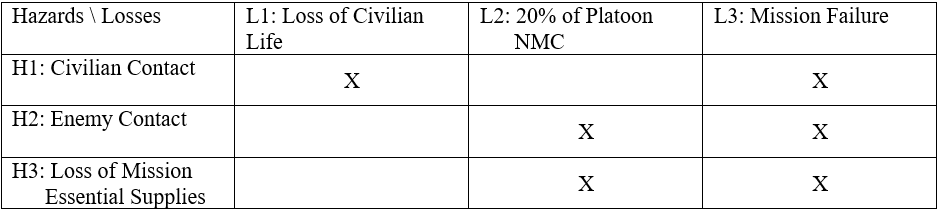
\includegraphics[scale=0.46]{HazardChart.PNG}
%   \caption{Hazard--Loss Table}
% \end{figure}

% Our functional control structure is the chain of command illustrated
% below outlines what individual, in what unit level would be
% responsible for the actions of the Soldiers below them.

% \begin{figure}[h]
%   \centering
%   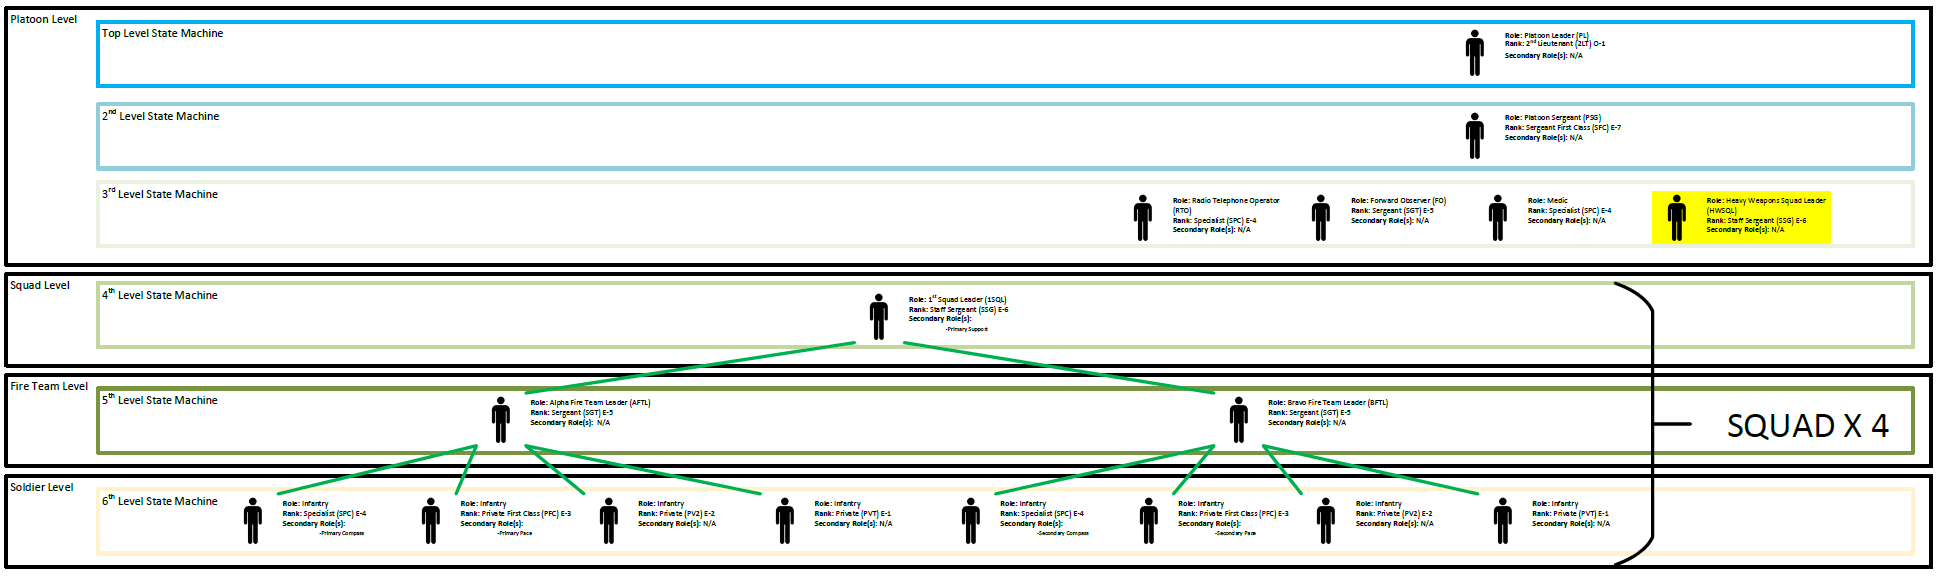
\includegraphics[scale=0.3]{OrganizationalChart.png}
%   \caption{Organizational Chart}
% \end{figure}

% The organizational chart showed the hierarchy of the Platoon and whom
% would be in control of each element and responsible for mitigating
% risks caused by hazards. Our application design recognized each
% leaders’ ability to control certain groups/units of Soldiers. With
% this in mind, leaders within the Platoon would have to (C1) avoid
% populated areas, (C2) avoid trafficked routes to and from those areas,
% (C3) maintain supplies within the HHQ standard operating procedure
% (SOP). These constraints were built into our application with states
% that performed reconnaissance, uniform and packing list checks,
% maintenance and cross loading of supplies.
